%% ****** Start of file aiptemplate.tex ****** %
%%
%%   This file is part of the files in the distribution of AIP substyles for
% %  REVTeX4.
%%   Version 4.1 of 9 October 2009.
%%
%
% This is a template for producing documents for use with
% the REVTEX 4.1 document class and the AIP substyles.
%
% Copy this file to another name and then work on that file.
% That way, you always have this original template file to use.

\documentclass[aip,graphicx]{revtex4-1}
%\documentclass[aip,reprint]{revtex4-1}
\usepackage[draft]{todonotes}

\draft % marks overfull lines with a black rule on the right

\begin{document}

% Use the \preprint command to place your local institutional report number 
% on the title page in preprint mode.
% Multiple \preprint commands are allowed.
\preprint{}

\title{Modeling vertical-axis cross-flow turbine wakes}

% repeat the \author .. \affiliation  etc. as needed
% \email, \thanks, \homepage, \altaffiliation all apply to the current author.
% Explanatory text should go in the []'s, 
% actual e-mail address or url should go in the {}'s for \email and \homepage.
% Please use the appropriate macro for the type of information

% \affiliation command applies to all authors since the last \affiliation command. 
% The \affiliation command should follow the other information.

\author{Peter Bachant}
\email[]{pxl3@unh.edu}
%\homepage[]{Your web page}
%\thanks{}
%\altaffiliation{}
\affiliation{Center for Ocean Renewable Energy, University of New Hampshire, 
Durham, NH}

\author{Martin Wosnik} 
%\email[]{}
%\homepage[]{Your web page}
%\thanks{}
%\altaffiliation{}
\affiliation{Center for Ocean Renewable Energy, University of New Hampshire,
Durham, NH}

% Collaboration name, if desired (requires use of superscriptaddress option in
% \documentclass).
% \noaffiliation is required (may also be used with the \author command).
%\collaboration{}
%\noaffiliation

\date{\today}

\begin{abstract}
The wake of a vertical-axis cross-flow turbine (CFT) is modeled numerically via
several techniques.
\end{abstract}

\pacs{}% insert suggested PACS numbers in braces on next line

\maketitle %\maketitle must follow title, authors, abstract and \pacs
\listoftodos

\section{Introduction}

In this study we set out to model the wake of the University of New Hampshire's
Reference Vertical-Axis (cross-flow) Turbine (UNH-RVAT) using a
Reynolds-averaged Navier--Stokes numerical model.

It has been shown that the momentum and energy transport processes in the
near-wake of a high-solidity, low aspect ratio vertical-axis turbine are
dominated by vertical advection \cite{Bachant2015-JoT}. It logically follows
that a 2-D simulation would not correctly predict wake recovery, but is of
interest to what extent this is true, since the computational feasibility of 2-D
simulations is attractive.

Modeling the boundary layer flows on cross-flow turbine blades is very
challenging due to the dynamically changing inflow and angle of attack---which
often exceeds static stall values and causes dynamic stall. Furthermore, the
ability to predict the occurrence and interdependence of boundary layer
transition and separation can have dramatic influence on the blade loading and
therefore the predicted turbine power output.

It is assumed that if the turbine power output and near-wake predictions from
the numerical model match those of the experiments, that the flow field can be
inspected in greater detail, i.e., that the experiments will have been
``interpolated''. This will allow us to see where the dominant flow structures
originate and help develop low-order wake generator models for use in turbine
array modeling. For example, Araya et al. modeled the flow through a VAT array
using leaky Rankine bodies \cite{Araya2014}. Shamsoddin and Porte-Agel modeled a
2-D CFT using large eddy simulation (LES) with an actuator line approach to
impart force on the flow field \cite{Shamsoddin2014}. 

Goude and Agren used a 2-D vortex method to simulate a farm of cross-flow
turbines \cite{Goude2010}. Durrani et al. used 2-D CFD to model a group of
cross-flow turbines, but did not compare with experimental results
\cite{Durrani2011}.

Questions addressed:

\begin{enumerate}

    \item Can 2-D RANS be used for array design?

    \item Does 3-D RANS tell us more about what is happening, i.e, can it
    ``interpolate'' the experimental results?
    
    \item Does 3-D RANS realize the proper wake recovery proportions? This would
    imply it could be a very accurate model if used in DES.

\end{enumerate}

Goals:

\begin{enumerate}

    \item Evaluate modern computational fluid dynamics techniques for predicting
    the dynamic loading on cross-flow turbine blades.

    \item If possible, accurately predict the turbine from the perspective as a
    wake generator, such that the results can be used to develop low-order
    models.

\end{enumerate}


\section{Numerical models}

The flow field was modeled using the Reynolds-averaged Navier--Stokes equations,
employing two different turbulence models--Menter's $k$--$\omega$ SST
\cite{Menter1994} and the Spalart--Allmaras (SA) one equation model
\cite{Spalart1992}. The SST model was chosen due to its prominence in the
literature for simulating separating flows, which we assumed to be present in
the current problem in the form of dynamic stall. The SA model was shown by
Ferreira et al. \cite{Ferreira2007} to match experimental particle image
velocimetry (PIV) results for a CFT in dynamic stall, though this was a somewhat
low Reynolds number case ($5 \times 10^4$).

\subsection{Computational mesh}

The computational domain is a rectangular volume 3.66 m long, 3.66 m wide, and
2.44 m tall (for 3-D), with the turbine located 1.52 m from the inlet, and
centered vertically with a vertical axis. with a cylindrical sliding mesh
interface, where the turbine zone rotates at a mean tip speed ratio
$\lambda=1.9$ with a sinusoidal oscillation at the blade passage
frequency---with and amplitude of 0.19 and the first peak at 0.7 radians---to
mimic the experimental data. The 2-D mesh is shown in Figure~\ref{fig:mesh}.

Meshes were generated using \textit{OpenFOAM}'s \textit{blockMesh} and
\textit{snappyHexMesh} utilities. Mesh topology consists of a background
hexahedral mesh, which is refined in all three directions by a factor of 2 in a
rectangular region containing the turbine and near-wake (0.9 m upstream, 1.3 m
downstream, $\pm 0.9$ m cross-stream, and $\pm 0.8$ m vertically). Cells
adjacent to the turbine shaft and struts are refined by a factor of 4, while
cells adjacent to the blades are refined by a factor of 6. To capture the
boundary layer, 20 layers are added next to the blades with an expansion ratio
of 1.2. Overall mesh refinement is controlled by a single parameter---the number
of cells in the streamwise direction, $N_x$.

3-D computer aided design (CAD) files of the turbine are available from
\cite{Bachant2014-RVAT-CAD}.

\begin{figure}[ht]
\caption{Snapshot of the 2-D computational mesh.}
\label{fig:mesh}
\end{figure}

\subsection{Software}

Simulations were run using the \textit{pimpleDyMFoam} solver from the
open-source finite volume CFD package \textit{OpenFOAM}, version 2.3.x.

\subsection{Initial and boundary conditions}

Initial and boundary conditions were set to match those of the tow tank as well
as possible. 

For the SA model, the turbulence transport variable $\tilde{\nu}$, is ideally
zero in the free stream \cite{Spalart1992}, though others recommend using
$\tilde{\nu}/\nu \approx 3$--$5$ for fully turbulent simulations
\cite{Spalart2007}. 

\section{Model verification}

The $k$--$\omega$ SST and Spalart--Allmaras RANS model cases were verified for
convergence of the turbine mean power coefficient with respect to grid spacing
and timestep. The grid topology was fixed, but the number of cells per unit
length were scaled proportionally, maintaining the same background mesh cell
aspect ratio. Results for this parameter sweep are shown in 
Figure~\ref{fig:spatial-grid-dep}, from which the final number of streamwise
grid points $N_x = 70$ was chosen. This corresponds to a total cell count of approximately $5 \times 10^4$ for the 2-D cases and 
\todo[inline]{Get total cell count for 3-D case.}

\begin{figure}[ht]
\caption{Spatial grid dependence for the SST (a) and Spalart--Allmaras (b) 
turbulence models for fixed timesteps.}
\label{fig:spatial-grid-dep}
\end{figure}

Timestep dependence was studied using the $N_x=70$ grid, the results from which
are shown in Figure~\ref{fig:timestep-dep}. It was seen that the
Spalart--Allmaras model converged well with decreasing timestep, leading to a
final timestep of 0.001 s. The results from the SST model show a local minimum,
at $\Delta t = 0.002$ s, which was the final timestep chosen to run the
simulations.

\begin{figure}[ht]
\caption{Spatial grid dependence for the SST (a) and Spalart--Allmaras (b) 
turbulence models for a grid with $N_x=70$.}
\label{fig:timestep-dep}
\end{figure}

\section{Model validation}

Models were validated against several open datasets.


\section{Results}

Computations for the 3-D cases were run on 192 processes and took on the order
of 1,000 CPU hours per second of simulation time. The 2-D simulations were run
on a single processor and took on the order of one CPU hour per second.


\subsection{Performance prediction}

Predictions for both the mean rotor power and drag coefficients are shown in
Figure~\ref{fig:perf-comp}. In general, the 2-D CFD cases both overpredict
turbine loading, which is likely due to their increased blockage ratio,
unresolved blade end effects, and lack of blade support struts.

The 3-D simulations fair better at predicting the experimental measurements,
with the Spalart--Allmaras model performing relatively better. The apparent
overprediction of rotor drag coefficient could be an effect of the experimental
procedure, where the ``tare drag'' from the turbine mounting structure was
measured without a turbine installed, then subtracted in post-processing.
Technically the local flow field will have changed, and hence the tare drag will
change as well.

\begin{figure}[ht]
    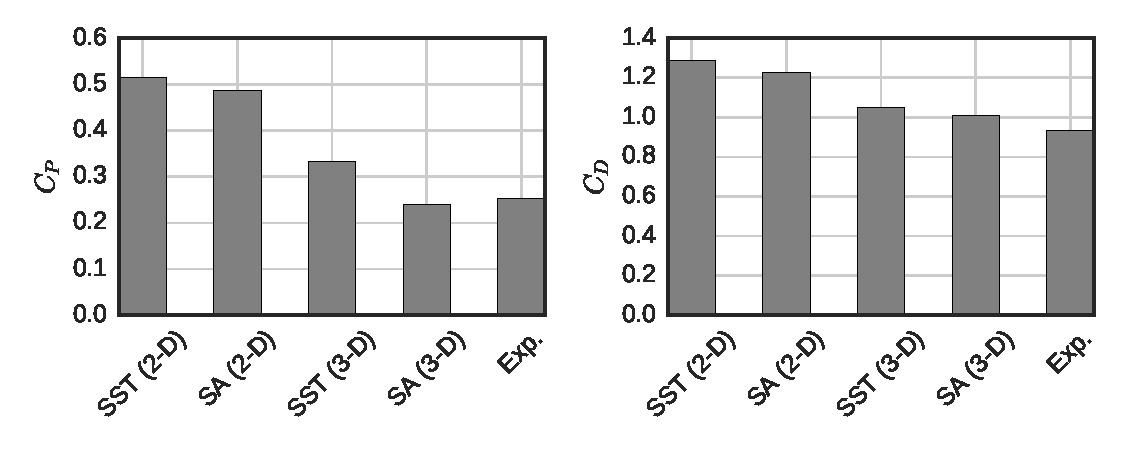
\includegraphics[width=0.9\textwidth]{figures/perf_bar_chart} \caption{Power
        (left) and drag (right) coefficient predictions from experiments and each
        numerical model.} \label{fig:perf-comp}
\end{figure}


\subsection{Wake characteristics}

Mean velocity profiles at one turbine diameter downstream are shown in
Figure~\ref{fig:profiles}. The 2-D results suffer from a blockage
mismatch, i.e. keeping the proximity of the walls constant increases the
blockage ratio.

\begin{figure}
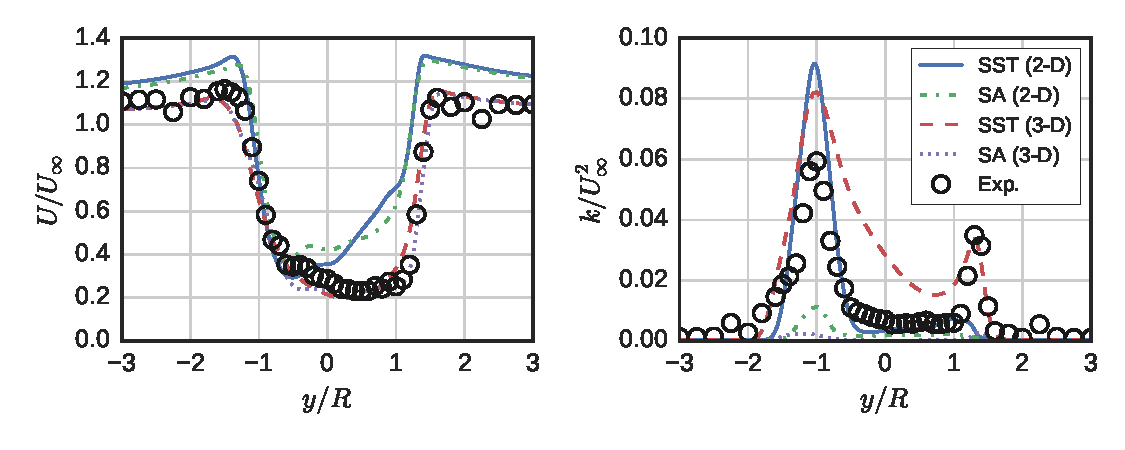
\includegraphics[width=0.95\textwidth]{figures/profiles} \caption{Mean velocity
	(left) and turbulence kinetic energy (right) profiles at $x/D=1$ from 2-D
	simulations, 3-D simulations ($z/H=0$), and experiments \cite{Bachant2015-JoT}.}
\label{fig:profiles}
\end{figure}

Turbulence kinetic energy profiles are also shown in Figure~\ref{fig:profiles}.
The turbulence kinetic energy is calculated as
\begin{equation}
k = k_{\mathrm{RA}} + \frac{1}{2} \left( 
\overline{U^\prime}^2 + 
\overline{V^\prime}^2 + 
\overline{W^\prime}^2 \right),
\label{eq:k}
\end{equation}
where $U^\prime = U - \overline{U}$ and $k_{\mathrm{RA}}$ is the kinetic energy
calculated by the turbulence model, which is zero for the SA model. Note that
the statistics of the Reynolds-averaged velocity are calculated from a time
series that has been downsampled to 50 Hz. It is assumed that this is far enough
from the blade passage frequency that differences from the variance in the
original velocity will be negligible.

We see that the side of the turbine with the upwind facing blade ($+y$), despite
having regions of high turbulence intensity, is actually more dominated by
unsteadiness in the Reynolds-averaged velocity, rather than the model's
turbulence kinetic energy.

\subsubsection{Momentum recovery}

To get an overall idea of the wake recovery predicted by each model, we
rearrange the streamwise component of the Navier--Stokes equation to isolate
$\partial U / \partial x$---following Bachant and
Wosnik\cite{Bachant2015-JoT}---and compute each term at $X/D = 1$ to compare
with the experimental results.

\begin{figure}[ht]
    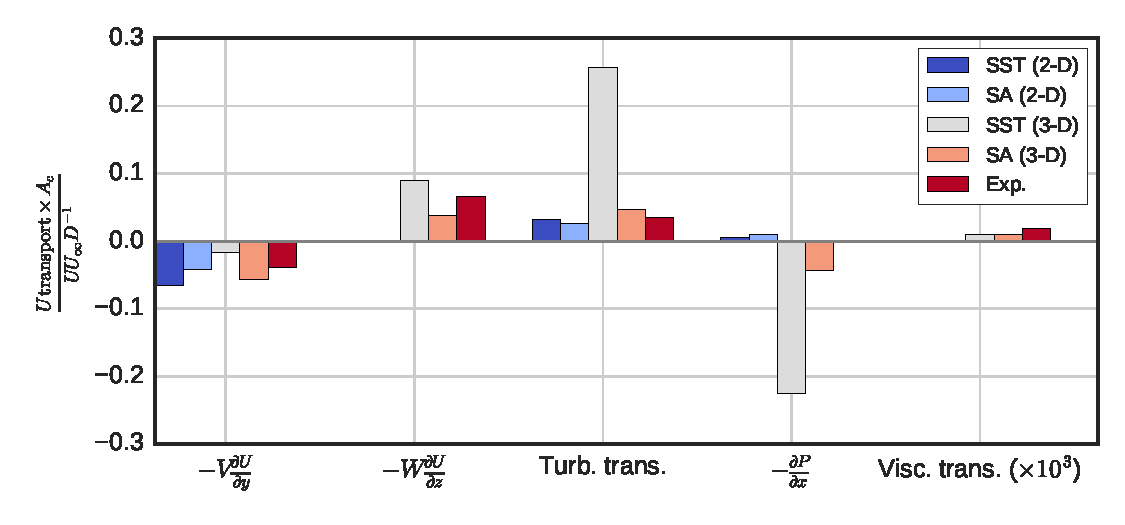
\includegraphics[width=0.9\textwidth]{figures/mom_bar_graph}
    \caption{Weighted sum normalized momentum recovery terms for each CFD case
        and experiments\cite{Bachant2015-JoT} at $x/D=1$.} \label{fig:recovery}
\end{figure}


\begin{acknowledgments}
The authors acknowledge Vincent Neary and the Sandia National Laboratories Water
Power Program for use of their Red Mesa high performance computing cluster.
\end{acknowledgments}

% Create the reference section using BibTeX:
\bibliography{library}

\end{document}
